\scanpage{34}

(namely the quotient by the image of $\Pi_2(Y)$),
and even by $\Pi_1(\mathcal V^*_{z,Z})$ itself if $\Pi_2(Y)$ is
zero. If we assume for simplicity\\
\hspace{.25cm}{\small\deleted{\unsure{cyclic}}}\\[-.35em]
that $\Pi_2(Y)\begin{tikzpicture}[baseline=-.35ex,x=1cm,y=1cm]
\draw[line width=.35pt] (0,0) -- (.53,.01) -- (.56,.055) -- (.60,-.035);
\end{tikzpicture}\Pi_1(\mathcal V^*_{z,Z})$ is zero, we find
therefore a diagram which makes (10) more precise

\diagram{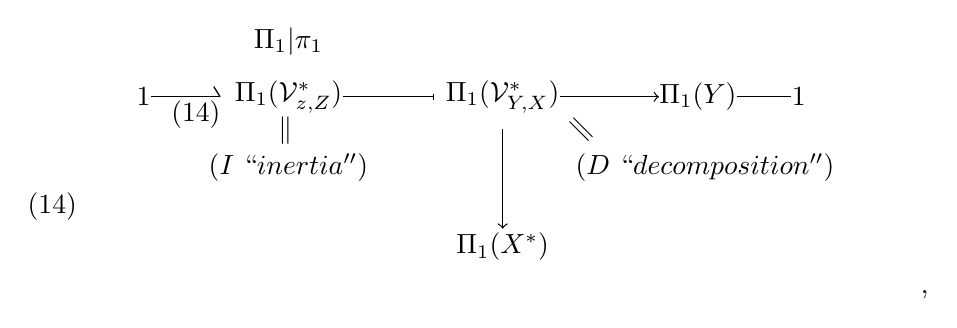
\begin{tikzpicture}[x=.8cm,y=.9cm]
\node[inner sep=0pt] (one) at (0,0) {$1$};
\node[inner sep=0pt] (fibre) at (2.3,0) {$\Pi_1(\mathcal V^*_{z,Z})$};
\node[inner sep=0pt] (middle) at (5.7,0) {$\Pi_1(\mathcal V^*_{Y,X})$};
\node[inner sep=0pt] (base) at (8.8,0) {$\Pi_1(Y)$};
\node[inner sep=0pt] (last) at (10.4,0) {$1$};
\draw[line width=.45pt] (one.east) -- ([xshift=-.18cm]fibre.west);
\draw[line width=.45pt] ([xshift=-.18cm]fibre.west) -- ([xshift=-.26cm,yshift=.13cm]fibre.west);
\draw[line width=.45pt] (fibre.east) -- ([xshift=-.15cm]middle.west);
\draw[line width=.45pt] ([xshift=-.15cm,yshift=.04cm]middle.west) -- ([xshift=-.15cm,yshift=-.04cm]middle.west);
\draw[->,line width=.45pt] (middle.east) -- (base.west);
\draw[line width=.45pt] (base.east) -- (last.west);
\node[inner sep=0pt] (bottom) at (5.7,-2.12) {$\Pi_1(X^*)$};
\draw[->,line width=.45pt] ([yshift=-.20cm]middle.south) -- ([yshift=.05cm]bottom.north);
\node[inner sep=0pt] at (2.25,-.48) {$\Vert$};
\node[inner sep=0pt] at (2.3,-1.00) {$(I\ \text{``inertia''})$};
\node[inner sep=0pt,rotate=45] at (6.95,-.46) {$\Vert$};
\node[inner sep=0pt,anchor=west] at (6.85,-1.00) {$(D\ \text{``decomposition''})$};
\node[inner sep=0pt] at (2.3,.78) {$\deleted{\unsure{\Pi_1|\pi_1}}$};
\node[inner sep=0pt] at (.83,-.25) {$\deleted{\unsure{(14)}}$};
\node[inner sep=0pt] at (-1.45,-1.55) {$(14)$};
\node[inner sep=0pt] at (12.4,-2.80) {,};
\end{tikzpicture}}

where the horizontal row is exact.

An interesting case is that where the
``building blocks'' which \deleted{\unsure{are}} occur,
namely $Y$, $X^*$ and $\mathcal V^*_{Z,z}$, are spaces
``$K(\Pi,1)$'', i.e.
\[
(15)\qquad \Pi_i(Y),\ \Pi_i(X^*),\ \Pi_i(\mathcal V^*_{Z,z}]\quad\text{zero for }i\geq 2,
\]
then we deduce that the same holds
for $\mathcal V^*_{Y,X}$ (and of course for $\mathcal V^*_{Y,X}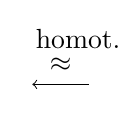
\begin{tikzpicture}[baseline=0pt,x=1cm,y=1cm]
\path[use as bounding box] (-.42,-.05) rectangle (.63,.72);
\draw[<-,line width=.35pt] (-.36,0) -- (.36,0);
\node[inner sep=0pt] at (0,.25) {$\approx$};
\node[inner sep=0pt] at (.22,.58) {$\mathrm{homot.}$};
\end{tikzpicture}Y$).
If we have the ``flexible \unsure{theory|Theory} of \uline{links} of
homotopy types'' to which I was making

\margin{33}
